% ***********************************************************
% ******************* PHYSICS HEADER ************************
% ***********************************************************
% Version 2
\documentclass[11pt]{article} 
\usepackage{amsmath} % AMS Math Package
\usepackage[utf8]{inputenc}
\usepackage[T1]{fontenc}
\usepackage{subfiles}
\usepackage{hyperref}
\usepackage{amsthm} % Theorem Formatting
\usepackage{amssymb}	% Math symbols such as \mathbb
\usepackage{graphicx} % Allows for eps images
\usepackage{multicol} % Allows for multiple columns
\usepackage[dvips,letterpaper,margin=0.75in,bottom=0.5in]{geometry}
 % Sets margins and page size
\pagestyle{empty} % Removes page numbers
\makeatletter % Need for anything that contains an @ command 
\renewcommand{\maketitle} % Redefine maketitle to conserve space
{ \begingroup \vskip 10pt \begin{center} \large {\bf \@title}
	\vskip 10pt \large \@author \hskip 20pt \@date \end{center}
  \vskip 10pt \endgroup \setcounter{footnote}{0} }
\makeatother % End of region containing @ commands
\renewcommand{\labelenumi}{(\alph{enumi})} % Use letters for enumerate
% \DeclareMathOperator{\Sample}{Sample}
\let\vaccent=\v % rename builtin command \v{} to \vaccent{}
\renewcommand{\v}[1]{\ensuremath{\mathbf{#1}}} % for vectors
\newcommand{\gv}[1]{\ensuremath{\mbox{\boldmath$ #1 $}}} 
% for vectors of Greek letters
\newcommand{\uv}[1]{\ensuremath{\mathbf{\hat{#1}}}} % for unit vector
\newcommand{\abs}[1]{\left| #1 \right|} % for absolute value
\newcommand{\avg}[1]{\left< #1 \right>} % for average
\let\underdot=\d % rename builtin command \d{} to \underdot{}
\renewcommand{\d}[2]{\frac{d #1}{d #2}} % for derivatives
\newcommand{\dd}[2]{\frac{d^2 #1}{d #2^2}} % for double derivatives
\newcommand{\pd}[2]{\frac{\partial #1}{\partial #2}} 
% for partial derivatives
\newcommand{\pdd}[2]{\frac{\partial^2 #1}{\partial #2^2}} 
% for double partial derivatives
\newcommand{\pdc}[3]{\left( \frac{\partial #1}{\partial #2}
 \right)_{#3}} % for thermodynamic partial derivatives
\newcommand{\ket}[1]{\left| #1 \right>} % for Dirac bras
\newcommand{\bra}[1]{\left< #1 \right|} % for Dirac kets
\newcommand{\braket}[2]{\left< #1 \vphantom{#2} \right|
 \left. #2 \vphantom{#1} \right>} % for Dirac brackets
\newcommand{\matrixel}[3]{\left< #1 \vphantom{#2#3} \right|
 #2 \left| #3 \vphantom{#1#2} \right>} % for Dirac matrix elements
\newcommand{\grad}[1]{\gv{\nabla} #1} % for gradient
\let\divsymb=\div % rename builtin command \div to \divsymb
\renewcommand{\div}[1]{\gv{\nabla} \cdot \v{#1}} % for divergence
\newcommand{\curl}[1]{\gv{\nabla} \times \v{#1}} % for curl

\newcommand{\laplace}[1]{\Delta #1} % for laplacian
\newcommand{\eps}{\epsilon_0} % electric permittivity
\newcommand{\oneover}[1]{\frac{1}{#1}} % 1/thing
\newcommand{\dotproduct}[2]{\v{#1} \cdot \v{#2}} % for dotproduct
\newcommand{\crossproduct}[2]{\v{#1} \times \v{#2}} % for crossproduct
\newcommand{\fourierv}[1]{\tilde{\v{#1}}}
%aliases
\newcommand{\para}{\parallel}
\newcommand{\rot}[1]{\curl{#1}}

\let\baraccent=\= % rename builtin command \= to \baraccent
\renewcommand{\=}[1]{\stackrel{#1}{=}} % for putting numbers above =
\newtheorem{prop}{Proposition}
\newtheorem{thm}{Theorem}[section]
\newtheorem{lem}[thm]{Lemma}
\theoremstyle{definition}
\newtheorem{dfn}{Definition}
\theoremstyle{remark}
\newtheorem*{rmk}{Remark}

% ***********************************************************
% ********************** END HEADER *************************
% ***********************************************************
\usepackage[utf8]{inputenc}
\usepackage{graphicx}
\title{Notes from PlasmaX}
\author{Dominik `Perfi' Stańczak}

\begin{document}
\maketitle

These notes will not be $100\%$ comprehensive, as I'm making them mainly for my own use. However, if you spot any mistakes, feel free to catch me on the forums and I'll fix any mistakes. 

\section{Week 1. Description of the plasma state, with Paolo Ricci}
Didn't start making notes until 1.5 so I'll be skimming the earlier topics.
	\subsection{Plasmas in nature and laboratory}
		\begin{itemize}
			\item Plasma - the 4th state of matter. Heat stuff up to ~11400K (= 1eV) and gases begin being ionized.
			\item The Sun is a miasma of incandescent plasma\footnote{\text{https://www.youtube.com/watch?v=sLkGSV9WDMA}}
			\item Lightning is plasma (ionized air)
			\item Plasma diplays
			\item Nuclear fusion - can't really get there without turning stuff into plasma
	\item The word `plasma' comes from greek $\pi\lambda\alpha\sigma\mu\alpha$, which means `moldable substance' or `jelly', though it was mentioned on the forums that it might mean `living thing'... which is really fitting when you think about it
			\item A brief history:
				\begin{itemize}
					\item 1920's-1930's: ionospheric plasma research (for radio transmission) and vacuum tubes (Langmuir)
					\item 1940's: MHD plasma waves (Alfvén)
					\item 1950's: research on Magnetic Fusion. Geneva UN conference on uses for atomic energy which don't kill people
				\end{itemize}
			\item Fusion experiments: L-1, TFTR, JET, ITER tokamaks; W7-X stellarator at MPI in Germany; the NIF inertial fusion facility in US
			\item The Earth's magnetosphere; van Allen belts
			\item Jets - space plasmas
			\item Lots of industrial applications
		\end{itemize}
		
	\subsection{Rigorous definition of plasma: Debye length}
	A plasma is a \textbf{globally neutral} \emph{ionised gas} with \textbf{collective effects}

	The following parameters classify plasmas:
		\begin{itemize}
			\item \textbf{Debye length}
			
			Distance over the potential of a charged particle decreases by a factor $1/e$ due to screening by other charged particles
			
			\[\lambda_{De} = \sqrt{\frac{\epsilon_0 T_e}{e^2 n_0}} \] (for electrons)
			
			Solved in lecture by a statistical approach which assumed $n\frac{4}{3}\pi \lambda_{De}^3 \equiv N_D \gg 1$ (for a Debye sphere; in the lecture $n \lambda_{De}^3$ was used, which relates to a Debye cube. There's not much difference between them, a factor of $~4$). $N_D$  means the number of particles inside a sphere (or cube, following the lecture) of radius equal to the Debye length. The condition means there's plenty of particles to screen our test particle. This also assumed that binary interactions between particles were weak ($\frac{e \phi}{T_e} \gg 1$)
			\end{itemize}
	\subsection{Plasma definition: frequencies and parameters}
\begin{itemize}
\item \textbf{Plasma frequency}
Assume a plasma of same density of ions and electrons. Displace electrons by $\Delta x$. They begin to exhibit harmonic oscillations (for $\Delta x$ not too large). Newton's 2nd law gives
\[\dd{\Delta x}{t} + \frac{n_0 e^2}{\epsilon_0 m_e}\Delta x = 0\]
Can define plasma frequency
\[\omega_{pe}\equiv\sqrt{\frac{n_0 e^2}{\epsilon_0 m_e}}=\frac{v_{th,e}}{\lambda_{De}}\]
where $v_{th,e}$ denotes the thermal speed of electrons
\item \textbf{Collision frequency}
	
	The frequency of coulomb collisions between particles
	\[\nu_{coll} \equiv \frac{n_0 e^4}{16 \pi \epsilon_0^2 m_e^2 v_{th,e}^3}\]
	
	\item Size of plasma has to be much larger than its Debye length (or there's no quasineutrality)
	\end{itemize}
	
	\subsection{Particle motion in a static uniform magnetic field . Plasma magnetic properties} 
		\begin{itemize}
			\item Larmor radius - particles gyrate around the guiding center at this distance
			\[\rho \equiv \frac{m v_{\perp}}{\abs{q} B}\]
			\item Cyclotron frequency
			\[\omega_c \equiv \frac{v_{\perp}}{\rho} = \frac{\abs{q} B}{m}\]
			
			Particle rotation direction on their helical trajectory
			\begin{itemize}
			\item $q>0$ (`by default'): left hand rotation with respect to $\v{B}$
			\item $q<0$ (electrons): right hand rotation
			
			\item Magnetic moment
			\[\abs{\v{\mu}} \equiv I A = \frac{\abs{q}\omega_e}{2\pi} \pi \rho^2 = \frac{m v_{\perp}^2}{2 B} = \frac{E_{kin \perp}}{B}\]
			
			(direction opposite to B)
			is an adiabatic invariant for every particle; doesn't change under slow changes of factors involved in the equation for $\mu$. However, it will change through heat exchange, which usually operates on slower timescales than magnetic field changes (see 2c).
			
			Plasmas are diamagnetic (they reduce externally applied magnetic fields) (because of direction of $\mu$)
			\end{itemize}
		\end{itemize}

	\subsection{Particle motion in given electromagnetic fields: the drifts }
Static and uniform E and B fields. Particles under Lorentz force which can be decomposed as:
	\begin{itemize}
		\item Parallel direction: \[m\d{\v{v_{\parallel}}}{t}=qE_{\parallel}\]
	Uniform acceleration
		\item Perpendicular direction: \[m\d{\v{v_{\perp}}}{t}=q(\v{E_{\perp}} + \v{V_{	\perp}}\times\v{B})\]
	\end{itemize}
The many drifts in a plasma:
	\begin{itemize}
		\item $\v{E}\times\v{B}$ drift
		\begin{itemize}
			\item Perpendicular component averages out over gyroperiod
			\[\v{v_e}=\frac{\v{E_{\perp}}\times\v{B}}{B^2}\]
			\item This is a motion of the guiding center which is superposed over the gyromotion
			\item Does not depend on charge, neither in magnitude nor in direction (but gyromotion direction does)
			\item Guiding center moves over lines of constant electrostatic potential $\phi$ (the drift does not change the particle energy!)
			\item A generalization of this drift for any force: \[\v{v_F}=\frac{\v{F_{\perp}}\times\v{B}}{qB^2}\]
			\item For a gravitational force (say, space plasmas), this depends on charge. Separates positive and negative charges. Polarizes the plasma, creating a $\v{E}$ field and an $\v{E}\times\v{B}$ drift
		\end{itemize}
		
		\item Curvature drift
		\begin{itemize}
			\item \v{B} field curved, particle follows the B field - this happens through a centrifugal force
			\[\v{F_c}=\frac{m v_{\parallel}^2}{R_B^2} \v{R_B}\]
			\item This causes a drift:
			\[\v{v_d} = \frac{\v{F_c} \times \v{B}}{q B^2} = \frac{m v_{\perp}^2}{q B^2 R_B^2} (\v{R_B} \times \v{B})\]
		\end{itemize}
		
		\item Gradient drift $\grad{B} \perp \vec{B})$
		\begin{itemize}
		\item	Happens in changing (spatially) magnetic fields
		\[\v{v_{\grad{B}}} = \frac{m v^2}{2 q B^3} (\v{B} \times {\grad{B}} ) \]
			\item A derivation so complicated, it deserved a separate appendix.
			As particles gyrate, they move between regions of smaller and bigger B.
			This causes a drift in a direction perpendicular to both the B field and the gradient of its value
			We consider a small variation in B and expand B in a taylor series around $B_0$.
			
			Then we use that expansion to solve $m \d{\v{v}}{t} = q {\v{v} \times {B}}$, plugging in our expansion for B.
			
			We also decompose the velocity: an average $v_{0}$ and a small perturbation. $v_{0}$ is the solution to the equation for constant magnetic field $B_{0}$.
			
			We neglect the cross product of the two small perturbations and average over a gyroperiod.
			
			We use our knowledge of the solution for the static magnetic field (gyration in the plane perpendicular to B) to deal with the perpendicular velocities (x and y in this decomposition under the assumption that B is along z).
			
			The drift velocity is the perturbation described by the formula above for an arbitrary geometry of the problem.
		\end{itemize}
	\end{itemize}
	
	
	\subsection{Plasma confinement based on single particle motion. Magnetic mirrors, stellarators, tokamaks}
	\begin{itemize}
	\item How do you confine a plasma?
	
	\textbf{Charged} particles follow helical trajectories along B field. This confines them in the perpendicular direction. What about the parallel one?
	\item Can use open field lines. Take two circular coaxial electromagnets.
	
	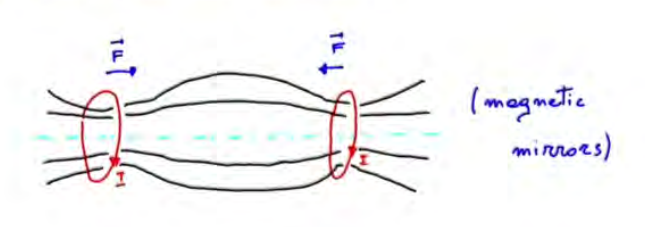
\includegraphics[width=\linewidth]{magneticmirror}
	
	\item Can use closed field lines. Closed geometries. Example: tokamaks (toroidal), stellarators.
	
	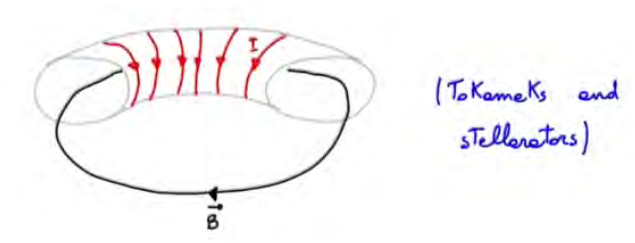
\includegraphics[width=\linewidth]{tokamakconfinement}
	
	\item The magnetic mirror geometry is neat for particles really close to the axis. B is maximum (field density increases) near the electromagnets
	
	force in the axial direction is \[F_z =-\mu\abs{\grad{B}}\]
	
	$v_{\parallel}$ has to vanish at $B_{max}$ so that the kinetic energy is just composed of the perpendicular component of velocity
	
	Particle reflection condition
	\[\frac{v_{\perp}^2}{v_{\perp}^2+v_{\parallel}^2} > \frac {B_{min}}{B_{max}}\]

	
	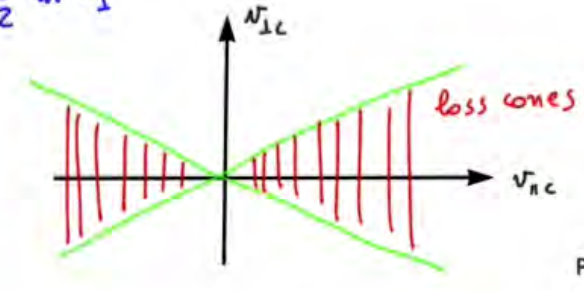
\includegraphics[width=\linewidth]{1f4}
	
	This means that particles in the \textbf{loss cones} in phase space (marked red; those which don't satisfy the inequality) cannot be confined in the mirror!
	
	Neat example: the Earth's magnetic field is a magnetic mirror!
	
	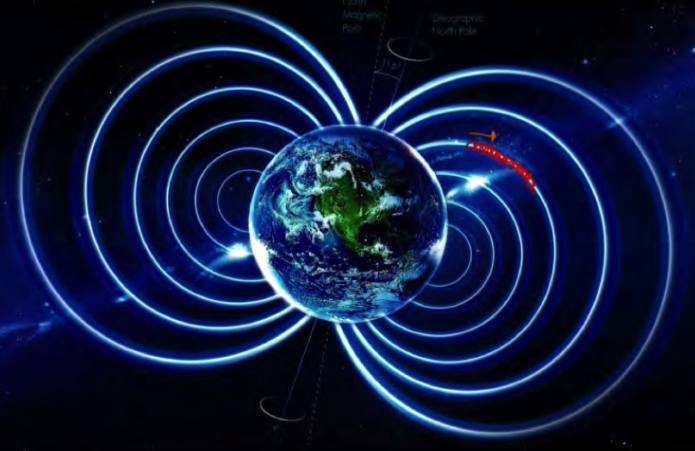
\includegraphics[width=\linewidth]{1f5}

\item What about closed magnetic field lines? Can those deal with loss cones?

B is not homogeneous! Curved! Has curvature and gradient drifts!

For a purely toroidal field, positively charged particles drift towards the bottom, while negatively charged ones drift towards the top. This polarizes the plasma and introduces the $E \times B$ drift outwards, sending the plasma crashing into the major radius wall.

A solution: a poloidal magnetic field to short circuit the charge accumulation. Either:
\begin{itemize}
\item Drive a current through the plasma $\rightarrow$ Tokamaks
\item Get rid of axial symmetry $\rightarrow$ Stellarators
\end{itemize} 

	
	\end{itemize}

%%WEEK 2%%
\section{Week 2: Kinetic description of plasmas, with Paolo Ricci}
\subsection{2a) From single particle to kinetic description }
	Kinetic description of plasma. A (relatively?) complete description of plasma which covers both the particles and the fields evolving over time.

The usual diagram for a plasma description, seen often in simulations:
\begin{enumerate}
	\item Take Newton's equations using electric and magnetic fields \textbf{for all particles at all times} (use Lorentz force)
	\item Use positions and velocities to compute charge and current densities. Charge density given as sum over particles of their charges, localized through use of Dirac delta functions. Current density - similar, but multiplied by particle velocity vectors inside the sum.
	\item Take charge and current density, plug them into Maxwell equations, calculate E and B fields at positions
	\item Take calculated E and B fields and apply them as forces to particles. Repeat cycle until bored or simulation returns segmentation fault.
\end{enumerate}
But real plasmas involve on the order of $10^21$ particles for a fusion plasma. Too much strain on our computational abilities. Impractical. We use a distribution function:

$f(\v{r}, \v{v}, t) d\v{r} d\v{v} = $ number of particles at time t, in phase space volume $d\v{r} d\v{v}$ located at $\v{r}, \v{v}$. We have a separate distribution function $f_i$ for every species
\begin{itemize}
\item Total number of particles $N_S$ given by integral of distribution function over all positions and velocities (which covers all the phase space)
\item Number density of particles $n_s$ given by integral over all velocities for a given location $\v{r}$ 
\item Average velocity given by $\frac{1}{n_s} \int \v{v} f_i(\v{r}, \v{v}, t)  d\v{v}$
\end{itemize}
\par \textbf{Examples of distribution functions}
\begin{itemize}
	\item Maxwell-Boltzmann distribution function, for three dimensions
	\[ F_0(\v{v}) = n_0 (\frac{1}{2 \pi v_{thermal}})^{3/2} exp(-\frac{v^2}{2 v_{thermal}^2}) \] %insert equation
	In 1D, only the normalization of the distribution changes from the 3D case:
	\[ F_0(v) = n_0 (\frac{1}{2 \pi v_{thermal}})^{1/2} exp(-\frac{v^2}{2 v_{thermal}^2}) \]
	\item Monoenergetic beam in 1D
	\[ F_0(v) = n_0 \delta (v-v_0) \]
	\item Two counterstreaming beams in 1D (two-stream instability!)
	\[ F_0(v) = \frac{n_0}{2} [\delta (v-v_0) + \delta(v+v_0)] \]
\end{itemize}

\textbf{Conservation of particles number}

If there are no sources or sinks, we have the following condition for conservation of number of particles
\[ \d{f_s}{t} = -\nabla_{6D} \cdot (\v{u} f_s) \]
where we introduce the six-dimensional nabla operator because who's gonna stop us
\[ \nabla_{6D} = ( \d{}{x},\d{}{y},\d{}{z},\d{}{v_x},\d{}{v_y},\d{}{v_z}) = (\d{}{\v{r}}, \d{}{\v{v}}) \]
\[ \v{u} = (\d{\v{r}}{t}, \d{\v{v}}{t}) = (\v{v}, \frac{\v{F}}{m_s}) = (\v{v}, \frac{\v{F_{long range}} + \v{F_{short range}}}{m_s}) \] %insert

Long range forces - collective interactions. Short range forces - binary collisions (between individual particles, like you'd have in a gas).
Plugging these back into the particle conservation equation:
\[ \d{f_s}{t} = -\d{}{\v{r}} \cdot (\v{v} f_s) - \d{}{\v{v}} \cdot [\frac{\v{F_{long range}} + \v{F_{short range}}}{m_s} f_s] \]

\textbf{Boltzmann equation}
	We can improve on the previous equation. Start out with the expanded particle conservation equation:
	
\[ \d{f_s}{t} = -\d{}{\v{r}} \cdot (\v{v} f_s) - \d{}{\v{v}} \cdot [\frac{\v{F_{long range}} + \v{F_{short range}}}{m_s} f_s] \]

\begin{itemize}
	\item In the phase space approach, velocity is treated as a completely independent variable than v (though you could consider one as a derivative of the other). Thus $\d{}{\v{r}} \cdot (\v{v} f_s) = \v{v} \cdot	\d{f_s}{\v{r}}$
		\item long range force can be decomposed into electric field independent of v, and the  $\v{v} \times \v{B}$ term - perpendicular to v. Thus, $\d{}{\v{v}} \cdot [\v{F_{long range}} f_s] = \v{F_{long range}}\cdot\d{f_s}{\v{v}} $
	\item Plugging in:
	
	\[ \d{f_s}{t} = -\v{v}\cdot\d{f_s}{\v{r}} - \frac{\v{F_{long range}}}{m_s} \cdot \d{f_s}{\v{v}} - \d{}{\v{v}} \cdot (\frac{\v{F_{short range}}}{m_s} f_s) \]
	\item Can be rewritten as:
	
	\[ \d{f_s}{t} +\v{v}\cdot\d{f_s}{\v{r}} + \frac{\v{F_{long range}}}{m_s} \cdot \d{f_s}{\v{v}} = - \d{}{\v{v}} \cdot (\frac{\v{F_{short range}}}{m_s} f_s) \]
	
	Term on the right is called a `collision operator' $(\d{f}{t})_c$.	
	
\item And we get the \textbf{Boltzmann equation}:
	\[ \d{f_s}{t} +\v{v}\cdot\d{f_s}{\v{r}} + \frac{q_s}{m_s}(\v{E_{long range}} + \v{v} \times \v{B_{long range}}) \cdot \d{f_s}{\v{v}} = (\d{f_s}{t})_c \]
\end {itemize}

\[   \]

\subsection{2b) Coulomb collisions in plasmas. Bonus module.}
We use Boltzmann equation and look into the short range interactions

An electron with charge $-e$ approaches a positive ion (assumed immobile) with charge $Ze$. Electron trajectory changes.
$\v{v_e}$ - initial electron velocity
$b$ - impact parameter, shortest distance between extrapolated line of initial electron trajectory and ion position

\[\frac{\text{Coulomb interaction energy}}{\text{Kinetic energy}} \sim \frac{\frac{Ze^2}{4 \pi \epsilon_0 b}}{m_e v_e^2} \sim 1 \]
(similar to one so collision interaction is important)
\[b \sim \frac{Ze^2}{4 \pi \epsilon_0 m_e v_e^2} = b_{\pi/2} \]

Coulomb cross section: $\sigma_{\pi/2} = \pi b_{\pi/2}^2 = \frac{\pi Z^2 e^4}{(4 \pi \epsilon_0)^2 m_e^2 v_e^4}$

Collision frequency: $\nu_{\pi/2} = n_i v_e \sigma_{\pi_2} = frac{n_i \pi Z^2 e^4}{(4 \pi \epsilon_0)^2 m_e^2 v_e^3}$

Is this a correct estimate? Do collective small angle deflections matter in a plasma? How can we take the interaction with many particles into account properly? Average over all phase space somehow?

Take the electron-ion collision again.
Denote $\theta$ - angle between initial and final electron velocity.

Particles interact through Coulomb force. Angular momentum and energy - conserved (if electron is much lighter than ion, $\frac{m_e}{m_i} \ll 1$).

\[ tan(\theta/2) = \frac{b_{\pi/2}}{b} = \frac{Ze^2}{4 \pi \epsilon_0 m_e v_e^2 b} \]

$b_{\pi/2}$ - impact parameter at which collision deflects electron by $90^\circ$.

Cumulative effect for many collisions? Imagine electron moving towards ion cloud.

Due to symmetry we take $\avg{\Delta \v{v_{\perp e}}} =0$ but $\avg{\Delta \v{v_{\perp e}^2}} \neq 0$ . So magnitude could change, but there will be no preferred direction. $\perp$ stands for parallel to initial velocity.
\[\d{\avg{\Delta \v{v_{\perp e}^2}}}{t} =\int db n_i v_e 2 \pi b \]
(we integrate over all possible impact parameters
\[ \Delta \v{v_{\perp e}^2} = v_e^2 \sin{\theta}^2 = \Delta v_e^2 \tan{\theta/2}^2 [1+\tan{\theta/2}^2]^{-2} \]

Plugging into the integral:
\[\d{\avg{\Delta \v{v_{\perp e}^2}}}{t} =8 \pi n_i v_e^3 \int_0^{\lambda_D} \frac{(b_{\pi/2} / b)^2 b}{(1+(b_{\pi/2} / b)^2)^2} db \pi b \]
We neglect quantum effects (thus integrating from 0) and integrate up to Debye length as coulomb interactions are screened beyond it. Finally, we get:
\[\d{\avg{\Delta \v{v_{\perp e}^2}}}{t} = 8 \pi n_i v_e^3 b_{\pi/2}^2 \ln{\frac{\lambda_D}{b_{\pi/2}}} \text{(if $\lambda_D \gg b_{\pi/2}$} \]

Following section may have some 4`s swapped for $\Delta$`s. 
\begin{itemize}
\item Note that electrons do not lose much energy as $m_e \ll m_i$. Basically reflected balls from a wall. Thus
\[ v_e (\Delta v_{\parallel e}) + 0.5 \Delta v_{\perp e}^2 = 0\]
And
\[\d{\avg{\Delta v_{\parallel e}}}{t} = - 4 \pi n_i v_e^2 b_{\pi/2}^2 \ln{\frac{\lambda_D}{b_{\pi/2}}} \]
\item We define the coulomb logarithm: 
\[ \ln{\Lambda} \equiv \ln{\frac{\lambda_D}{b_{\pi/2}}} \sim \text{In most plasmas equals  15 to 25} \]
\item 
\[ \d{\avg{\Delta v_{\parallel e} }}{t} = - \nu_{ei} v_e \]
Collision frequency of electrons against ions:
\[ \nu_{ei} = 4 \pi n_i b_{\pi/2}^2 v_e \ln{\Lambda} = n_i \sigma_{ei} v_e \]
Whereas
\[ \sigma_{ei} = 4 \pi b_{\pi/2}^2 \ln{\Lambda} \]
Can compare 
\[ \frac{\sigma_{\pi/2}}{\sigma_{ei}} = \frac{\pi b_{\pi/2}^2}{4 \pi b_{\pi/2}^2 \ln{\Lambda}} \ll 1\]
Much smaller than 1! So small angle deflections dominate over large scale deflections!
\end{itemize}

\subsection{2c) Collisional processes in plasmas}
\subsubsection{Slowing down of an electron beam}
\[ \d{\avg{\Delta v_{\parallel e} }}{t} = - \nu_{ei} v_e = -\frac{n_i Z^2 e^4 \ln{\Lambda}}{4 \pi \epsilon_0^2 m_e^2 v_e^3} \]
We could use this to calculate how an electron beam slows in a plasma.
Assume a Maxwellian distribution of electron velocities with mean velocity $u_e\ll v_{thermal, e}$ in 1D:
\[ f_e(v) = n_0 (\frac{m_e}{2 \pi v_{thermal,e}})^{1/2} exp(-\frac{m_e (v_{\parallel e} - u_e)^2}{2 v_{thermal,e}^2}) \]

\[ \d{u_e}{t} = -\avg{\nu_{ei} v_{\parallel e}} = \frac{-1}{n_0} \int{\nu_{ei} v_{\parallel e} f_e(v_{\parallel e}) dv_{\parallel e}} \simeq -\avg{\nu_{ei}} u_e (\text{if } u_e \ll v_{thermal, e})\]  

The average collision frequency between electrons and ions $\nu_{ei}$ is

\[ \nu_{ei} = \frac{\sqrt{2}}{12 \pi^(3/2)} \frac{n_i Z^2 e^4 \ln{\Lambda}}{\epsilon_0^2 m_e^(1/2) T_e^(3/2)} \]

There are also collisions between electrons coming from the beam and electrons in the plasma:
\[ \nu_{ee} = \frac{\sqrt{2}}{12 \pi^(3/2)} \frac{n_e e^4 \ln{\Lambda}}{\epsilon_0^2 m_e^(1/2) T_e^(3/2)} \sim \frac{\avg{\nu_{ei}} n_e}{Z^2 n_i} \]

\subsubsection{Plasma resistivity}
Take a cloud of ions and electrons. Apply electric field $\v{E}$. Ions will move in direction of E, whereas electrons will move in opposite direction. E then drives a current in a plasma - charges are moving!

We neglect the slow and heavy electrons and focus on electron movement. From Newton's second law:

\[m_e n_e \d{\v{u_e}}{t} = -e n_e \v{E} + \v{R_{ei}} \]
$R_{ei}$ is the collision term we have just calculated. This slows down the current.
\[\v{R_{ei}} = - m_e n_e \avg{\nu_{ei}} (\v{u_e}-\v{u_i}) \text{ (assuming } u_e \ll v_{th,e} ) \]

\begin{itemize}
\item After a transient, we'll reach steady state operation and $\d{}{t}=0$
\item The current can be depicted as $\v{j} = - n_e e (\v{u_e}-\v{u_i})$
\end{itemize}
Thus:
\[ e^2 n_e \v{E} = m_e \avg{\nu_{ei}} \v{j}\]
\[ \v{E} = \frac{m_e \avg{\nu_{ei}}}{e^2 n_e} \v{j} \equiv \eta \v{j} \]
By comparison with Ohm's law we can define the plasma resistivity:
\[ \eta \equiv \frac{m_e \avg{\nu_{ei}}}{e^2 n_e} = \frac{ \sqrt{2 m_e} Z	e^2 \ln{\Lambda}}{12 \pi^{3/2} \epsilon_0^2 T_e^{3/2}} \]
The bigger the temperature, the lower the resistivity. Unlike in metals. It's also independent of density! The contributions of increasing the number of carriers and increasing the number of collisions cancel each other out exactly.
\subsubsection{Overview of plasma collision frequencies}
\begin{itemize}
\item Electron - ion collision frequency $nu_{ei} = $ 
\item Electron - electron collision frequency $nu_{ei}$
\item Ion - ion collision frequency $nu_{ii}$.
\end{itemize}

Ions gain energy when you fire an electron beam into a plasma (could be heated this way?).

\[ m_e \Delta \v{v_e} = m_i \Delta \v{v_i}\]
\[ 0.5 m_i \abs{\Delta \v{v_i}}^2 = \frac{ m_e^2}{2 m_i} \abs{\Delta \v{v_e}}^2 \sim \frac{m_e^2}{2 m_i} \abs{\Delta \v{v_{\perp e}}^2}\]
(as we can ignore the change in parallel electron velocity)

Rate of exchange of energy (between species! This equalizes the temperatures between electrons and ions!):
\[ \avg{\nu_E} = \frac{n_i Z^2 e^4 \sqrt{m_e} \ln{\Lambda}}{3 \pi \sqrt{2 \pi} \epsilon_0^2 m_i T_e^{3/2}} \sim Z \frac {m_e}{m_i} \avg{\nu_{ei}} \]

The electrons have a similar, very fast rate of collisions with each other and with ions. The rate of collisions between ions happens $~40$ times slower, and then the rate of energy exchange is $~40$ times slower than that. At a similar rate to that of energy exchange is the rate of ions colliding with electrons.

\subsection{2d) Vlasov equation}
\subsubsection{Derivation from Boltzmann equation}
\[\d{f_s}{t} + \v{v} \cdot \d{f_s}{\v{r}} + \frac{q_s}{m_s} (\vec{E} + \vec{v} \times \v{B}) \cdot \d{f_s}{\v{v}} = (\d{f_s}{t})_c\]
If we can assume that the number of particles in a Debye cube is REALLY HIGH: $n \lambda_D^3 \gg\gg$, so that  $(\d{f}{t})_c=0$, then the \textbf{Vlasov equation} holds:
\[\d{f_s}{t} + \v{v} \cdot \d{f_s}{\v{r}} + \frac{q_s}{m_s} (\vec{E} + \vec{v} \times \v{B}) \cdot \d{f_s}{\v{v}} = 0\]
E and B here represent the long range interactions. The charge density is computed as indicated before, integrating out all the velocities. The currents are likewise obtained by summing over the species and calculating the average velocities at each positions.

\subsubsection{Conservation laws for the Vlasov equation}
\[\d{f_s}{t} + \v{v} \cdot \d{f_s}{\v{r}} + \frac{q_s}{m_s} (\vec{E} + \vec{v} \times \v{B}) \cdot \d{f_s}{\v{v}} = 0\]
This satisfies the following conservation properties:
\begin{itemize}
\item Number of particles - we can integrate the Vlasov equation over all positions and velocities. Integrating $\d{f_s}{t}$ gives us $\d{N_s}{t}$. The second term gives us, by means of Gauss (divergence) theorem and pushing the boundaries out to infinity, where $f_s$ should decay to zero, zero. In the third term we have a velocity divergence. Since no particles have infinite velocities\footnote{Einstein says hi.}, we can once more use the divergence theorem \textit{(in velocity space!!!)} to eliminate the third term and we reach $\d{N_s}{t} = 0$. Particles are conserved.
\item Momentum, which we calculate as the sum of particle and field momenta. No actual derivation is given except for the formula:

\[ \v{P_{tot}} = \sum_s m_s \int d\v{r} \int d\v{v} \, \v{v} f_s + \epsilon_0 \int d\v{r} (\v{E} \times \v{B}) = \text{const}  \]

\item Total energy can be decomposed into energy of particles and energy of field.
\[ E= \sum_s \int d\v{r} \int d\v{v} \frac{1}{2} m_s v^2 f_s + \frac{1}{2} \int d\v{r} (\epsilon_0 E^2 + B^2/\mu_0) = \text{const} \]

\item Entropy, as given by information theory
\[ S = \sum_s \int d\v{r} \int d\v{v} f_s \ln{f_s} = \text{const} \]
This is because collisions are neglected by the Vlasov equation. Therefore it is time-reversible!
\end{itemize}


\subsubsection{Interpretation of Vlasov equation}
\begin{itemize}
\item $f_s$ has incompressible motion (in phase space) - it can be considered as an incompressible fluid (moving in phase space - it's going to obey Liouville's theorem)
\item As seen by particle along orbit \[ \d{f_s}{t} = \pd{f_s}{t} + \v{v} \cdot \pd{f_s}{\v{r}} + \frac{\v{F}}{m_s} \cdot \pd{f_s}{\v{v}} = \pd{f_s}{t} + \v{v} \cdot \pd{f_s}{\v{r}} + \frac{q_s}{m_s} (\v{E} + \v{v} \times \v{B}) \cdot \pd{f_s}{\v{v}} \]
And the funny thing is, that's just the Vlasov equation itself. Thus along particle orbits, $f_s = 0$.
\end{itemize}

\subsubsection{(Formal) solutions of Vlasov equation}
If $c_j$ is a constant of motion, then any distribution function being a function of any number of constants of motion $c_j$  is a solution.

This is unlike the Boltzmann equation, where only the Maxwellian distribution was a stationary solution.

It can be really difficult to find constants of motion, as well. It seems to be implied that practical solutions rely on numerical methods - that way you need not specify constants of motion for a formal solution.

\subsection{The two stream instability!}
We make this our testing ground for the Vlasov equation. The situation is two beams of electrons moving in opposite directions in 1D. Spoiler alert - WE'RE ACTUALLY GOING TO MESS AROUND WITH THE MATLAB CODE FOR THIS KIND OF SIMULATION IN THE HOMEWORK, THIS IS AWESOME. Ahem.
\subsubsection{Simplifications}
We take the Vlasov equation and Maxwell's equations

\[\d{f_s}{t} + \v{v} \cdot \d{f_s}{\v{r}} + \frac{q_s}{m_s} (\vec{E} + \vec{v} \times \v{B}) \cdot \d{f_s}{\v{v}} = 0\]
\[ \div{\v{E}} = \frac{\rho}{\epsilon_0} \]
\[ \div{\v{B}} = 0 \]
\[ \curl{\v{E}} = -\d{\v{B}}{t} \]
\[ \curl{\v{B}} = \mu_0 ( \v{j} + \epsilon_0 \d{\v{E}}{t}) \]

We simplify the situation. Set $\v{B} = 0$ for an electrostatic situation.

\[\d{f_s}{t} + \v{v} \cdot \d{f_s}{\v{r}} + \frac{q_s}{m_s} \vec{E} \cdot \d{f_s}{\v{v}} = 0\]
\[ \div{\v{E}} = \frac{\rho}{\epsilon_0} \]
\[ \div{\v{B}} = 0 \]
\[ \curl{\v{E}} = 0 \]
which implies
\[\v{E} = -\grad{\phi}\]
\[\Delta\phi = -\frac{\rho}{\epsilon_0} \]

We also assume that ions are stationary in the background with density $n_0$ (electrons move at a much faster time scale). This means we only have to solve Vlasov for the electron motion and can replace $f_s$ by $f$ for brevity:

\[\d{f}{t} + \v{v} \cdot \d{f}{\v{r}} - \frac{e \vec{E}}{m_s} \cdot \d{f}{\v{v}} = 0\]
\[\Delta\phi = \frac{e}{\epsilon_0} \int f d\v{v} - \frac{e}{\epsilon_0} n_0\]

\subsubsection{Linearisation}

We're going to be analysing small perturbations from equilibrium. This means basically expanding the quality of interest in a short Taylor series:
\[g=g_0 \text{ (equilibrium)} + g_1 \text{ (perturbation, $g_1 \ll g_0$) } \]

In our case, $f_0$ being the initial distribution functions which is isotropic over all position space (thus no dependence on $\v{r}$) and $f_1$ being our small perturbation:
\[f(\v{r}, \v{v}, t) = f_0 (\v{v}) + f_1(\v{r}, \v{v}, t) \]
\[\phi = \phi_1 (\v{r}, t) \text{ as we can set $\phi_0 = 0$ since it's constant anyway} \]
\[\v{E} = \v{E_1} (\v{r}, t)\]

We plug these into the Vlasov equation:

\[ \pd{f_0 + f_1}{t} + \v{v} \cdot \pd {(f_0 + f_1)}{\v{r}} - \frac{e \v{E_1}}{m_e} \cdot \pd{(f_0 + f_1)}{\v{v}} = 0 \]

Simplifying and neglecting $\v{E_1} \cdot \pd{f_1}{\v{v}}$ as small times small:

\[\pd{f_1}{t} + \v{v} \cdot \pd{f_1}{\v{r}} - \frac{e\v{E_1}}{m_e} \cdot \pd {f_0}{\v{v}}\]

Also plugging in $\v{E_1} = -\grad{\phi}$:

\[ \Delta \phi_1 = \frac{e}{\epsilon_0} \int f_1 d\v{v} \]

Thus:

\[\pd{f_1}{t} + \v{v} \cdot \pd{f_1}{\v{r}} - \frac{e}{m_e}\pd{\phi_1}{\v{r}} \cdot \pd {f_0}{\v{v}}\]
\[ \Delta \phi_1 = \frac{e}{\epsilon_0} \int f_1 d\v{v} \]

We now apply Fourier analysis to $f_1$:

\[ f_1 (\v{r}, \v{v}, t) = \int d\v{k} \int d\omega \tilde{f_1} (\v{k}, \v{v}, \omega) \exp{i(\v{k} \cdot \v{r} - \omega t)} \]
This is neat because:
\begin{itemize}
\item The time derivative is simple:
\[ \pd{f_1}{t} (\v{r}, \v{v}, t) = \int d\v{k} \int d\omega (-i\omega) \tilde{f_1} (\v{k}, \v{v}, \omega) \exp{i(\v{k} \cdot \v{r} - \omega t)} \]
\item The spatial derivative is also pretty simple:
\[ \pd{f_1}{\v{r}} (\v{r}, \v{v}, t) = \int d\v{k} \int d\omega (i\v{k}) \tilde{f_1} (\v{k}, \v{v}, \omega) \exp{i(\v{k} \cdot \v{r} - \omega t)} \]
\end{itemize}

So we go back to the Vlasov equation and plug in the expressions above:

\[\pd{f_1}{t} + \v{v} \cdot \pd{f_1}{\v{r}} - \frac{e}{m_e}\pd{\phi_1}{\v{r}} \cdot \pd {f_0}{\v{v}} = 0\]
\[\int d\v{k} \int d\omega [(-i\omega + i \v{k} \cdot \v{v}) \tilde{f_1} + \frac{i e \tilde{\phi_1}}{m_e} \v{k} \cdot \pd{f_0}{\v{v}}]\exp{i(\v{k} \cdot \v{r} - \omega t)} = 0 \]

This can be true only if all the coefficients vanish:

\[ (-i\omega + i \v{k} \cdot \v{v}) \tilde{f_1} + \frac{i e \tilde{\phi_1}}{m_e} \v{k} \cdot \pd{f_0}{\v{v}} = 0 \]
\[ \tilde{f_1} = \frac{e}{m_e} \frac{\tilde{\phi_1}}{\omega - \v{k} \cdot \v{v}} \v{k} \cdot \pd{f_0}{\v{v}} \]

Plugging this result into the Fourier transform of the Poission equation above:

\[ \Delta \phi_1 = \frac{e}{\epsilon_0} \int f_1 d\v{v} \]
\[ -k^2 \tilde{\phi_1} = \frac{e}{\epsilon_0} \int \tilde{f_1} d\v{v} =\frac{e^2 \tilde{\phi_1}}{\epsilon_0 m_e} \int \frac{\v{k} \cdot \pd{f_0}{\v{v}}}{\omega - \v{k} \cdot \v{v}} d\v{v} \]

Which then implies

\[ \tilde{\phi_1} k^2 [ 1+ \frac{e^2}{\epsilon_0 m_e k^2} \int \frac{\v{k} \cdot \pd{f_0}{\v{v}}}{\omega - \v{k} \cdot \v{v}} d\v{v} ] =0 \]

We denote the bulky part as the dispersion function

\[ D(\omega, \v{k}) \equiv 1+ \frac{e^2}{\epsilon_0 m_e k^2} \int \frac{\v{k} \cdot \pd{f_0}{\v{v}}}{\omega - \v{k} \cdot \v{v}} d\v{v} \]

Which we can find the roots of, and the solutions (values of $\omega$ and $\v{k}$) gives us the normal modes of our plasma.

There's a singularity at $\omega = \v{k} \cdot \v{v}$. This is when particles match velocities with wave velocities in the plasmas... this may or may not be connected to Landau damping. This topic will not be further developed in the course.

\subsubsection{Getting to the two-stream instability}

The two-stream instability is thermodynamically weird. The velocity distribution is definitely non-maxwellian, it's just two sharp peaks (low entropy). Could there be intrinsic modes in the system that restore thermodynamic equilibrium (high entropy)?

We take a 1D system. The derivation above is general (plenty of vectors brought to you by yours truly). 

\[f=f_0(v_x) = f(u)\]

\[ D(\omega, k) = 1 + \frac{e^2}{\epsilon_0 m_e} \frac{1}{k} \int \d{f_0}{u} \frac{du}{\omega-k u} \]

I'm pretty sure there's a mistake in the lecture and a $1/k$ factor was lost there (it should be $1/k^2$).

For two counter streaming beams:

\[ f_0 (u) =\frac{n}{2} [\delta(u-v_0) + \delta(u+v_0)] \]

The distribution function `luckily' avoids the singularity. We calculate the dispersion function and arrive at

\[D(\omega, k) = 1- \frac{n e^2}{2 \epsilon_0}{m_e} [\frac{1}{(\omega-k v_0)^2} + \frac{1}{(\omega + k v_0)^2} ] \]

(note that the plasma frequency pops up: $\omega^2_{pe} = \frac{n e^2}{\epsilon_0 m_e}$)

This is a $4$th order polynomial in the nominator. The function has two vertical asymptotes at $\omega = \pm k v_0$ and a horizontal one at $1$.

Depending on the parameters, if $D(\omega=0, k) \geq 0$, there's $4$ real roots. The modes will be oscillatory instead of exponentially growing.

Otherwise, if $D(\omega = 0, k) < 0$, there's $2$ real roots corresponding to oscillations and $2$ complex roots corresponding to exponential explosions.

\[ D(\omega =0, k) = 1 - \frac{\omega_{pe}^2}{k^2 v_0^2} < 0 \rightarrow k^2 v_0^2 < \omega_{pe}^2 \]

Unstable modes are those that have sufficiently long wavelengths. That's all we can tell analytically. IT'S PARTICLE IN CELL TIME!
\end{document}